\chapter{Superconductivity}
The theory of superconductivity was formulated by Bardeen, Cooper, and Schrieffer (1957) and is called the BCS theory.
It very successfully describes the superconducting properties of weak superconductors, such as aluminum, which are weak because of the small strength of electron-phonon interaction.
Further refinement of the theory have led to strong coupling theory of Eliashberg, which describes the properties of superconductor lead.
The distinction is roughly determined by the value of the electron-phonon mass enhancement factor $\lambda$ shown by McMillan.

The basic idea of BCS theory is that the electrons in the metal form bound pairs.
This bound states of electron pairs are not described by simple orbitals such as hydrogen atom.
The pair state and entire ground state of the superconductor requires a many-body description.

Fr{\"o}hlich was the first to realize that electrons could interact by exchanging phonons and that this interaction could be attractive.
Another piece in theoretical puzzle was supplied by Schafroth, who shown that a charged boson gas, when undergoing a Bose-Einstein condensation would exhibit many of superconducting properties such as Meissner effect.
In the BCS theory, the electron pairs behave in some respects as bosons.

\section{Cooper Instability} \label{se:10.1}
Cooper pointed out that the ground state of a normal metal was unstable at zero temperature.
A normal metal is defined as one which is neither superconducting nor magnetic.
The demonstration of an instability does not provide a description of superconducting state, but it suggest that the instability was caused by the scattering between pairs of electrons, where the scattering potential is the exchange of phonons.

The scattering process as shown \ref{fig:10.1}.
\begin{figure}[ht]
    \centering
    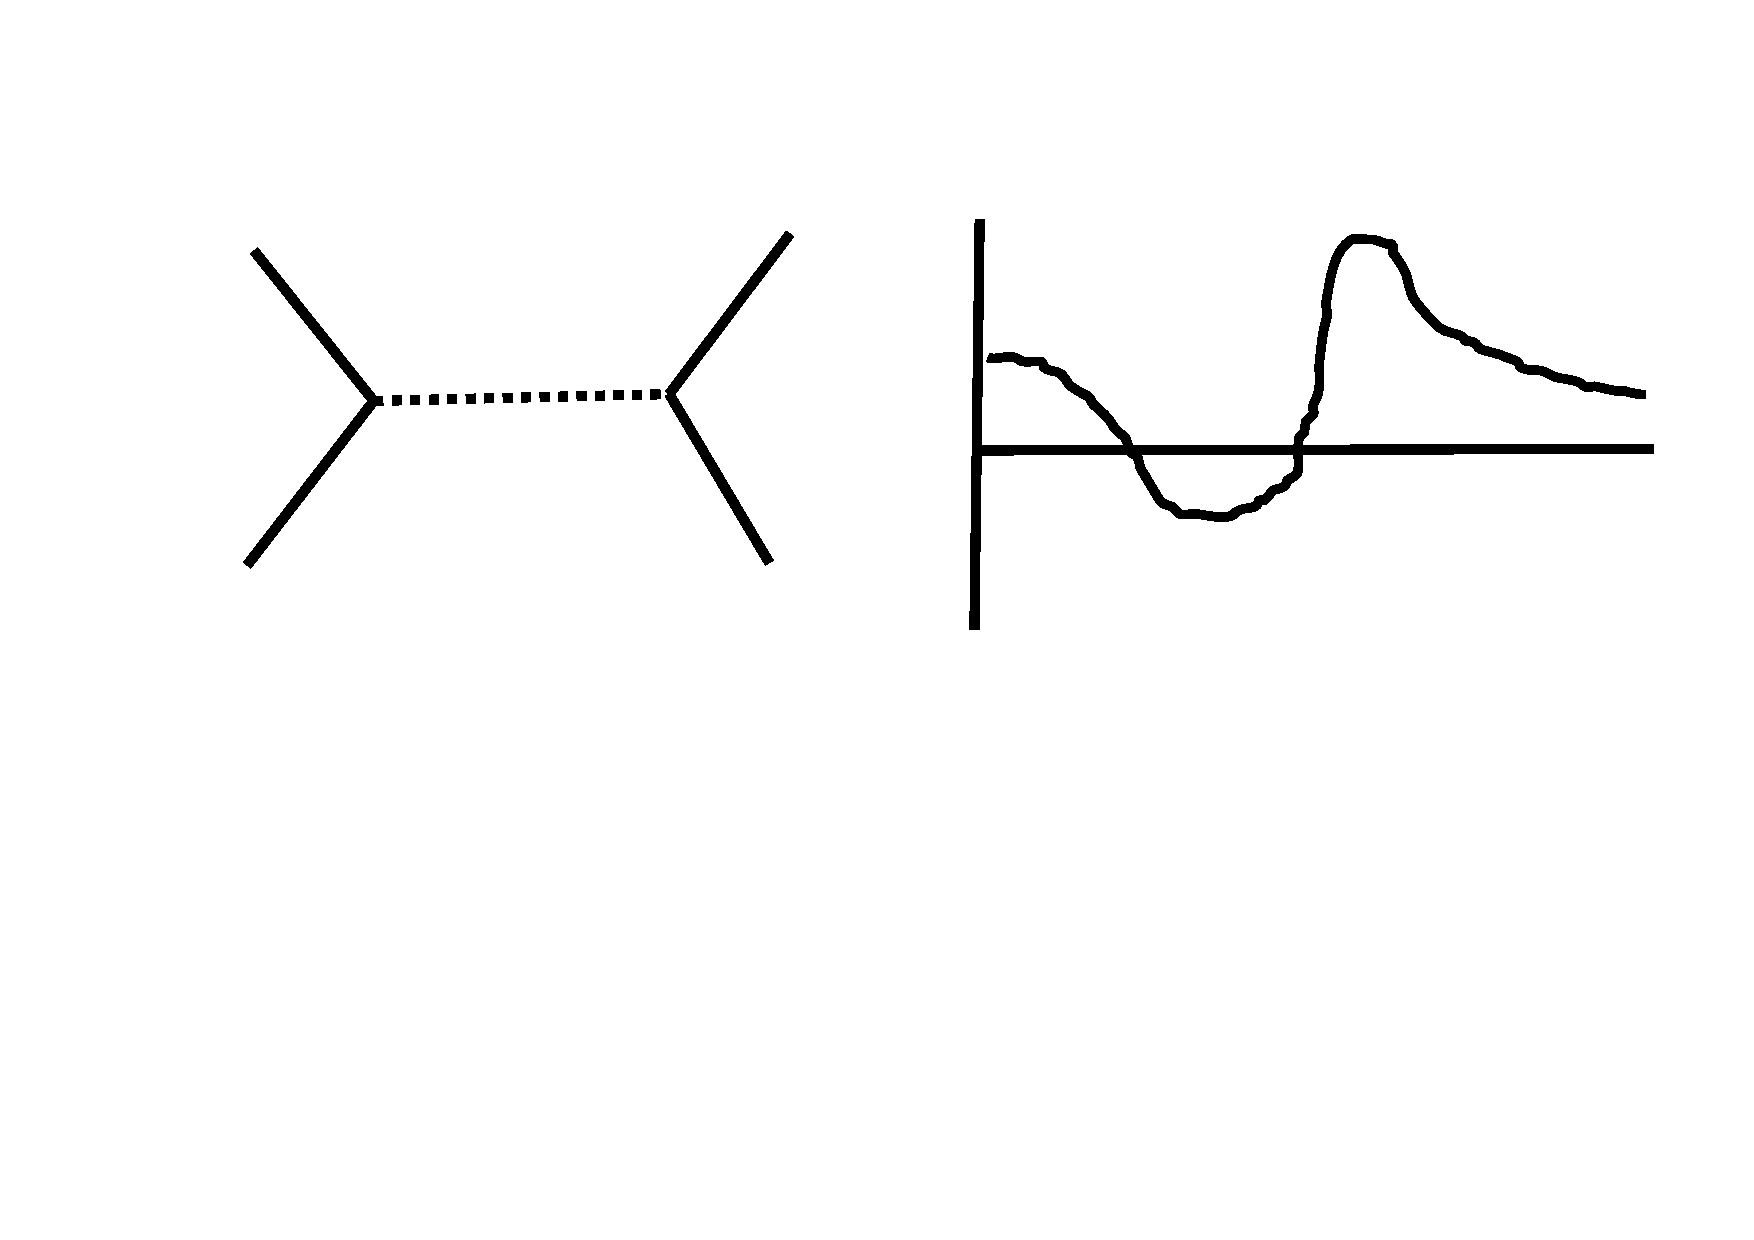
\includegraphics[width=0.8\linewidth]{./fig/fig10_1.pdf}
    \caption{Scattering process and potential}%
    \label{fig:10.1}
\end{figure}
The screened interaction between two electrons was derived before as
\begin{equation}
    V_s(\bq,\omega) = \frac{v_q}{\varepsilon(\bq,\omega)}  + \frac{2\omega \lambda M^2_\bq}{\varepsilon(\bq)^2 \left[ \omega^2 - \omega_\lambda(\bq)^2\right]}  \label{10.1}
\end{equation}
The first is the screened Coulomb interaction.
The theory of superconductivity is applied at low temperatures, where the energy exchanged between particles, while scattering, is also low.
The requirements of crystal stability require that this interaction be repulsive at zero frequency.

The second term in \eqref{10.1} is the screened electron-phonon interaction.
It is on the average weaker than the repulsive Coulomb interaction.
However, for frequency near to Debye $(\omega <\omega_D)$ the energy denominator becomes small and negative, which causes a relatively large interaction over this narrow range of frequency.
It may be possible for two electrons to bind if they can construct a relative wave function which selectively uses the frequency region which is attractive.

For simplicity instead of \eqref{10.1} use a interaction model
\begin{equation}
    V_s(\bq,\omega) =
    \begin{cases}
        -V_0 ~ ~&  \abs{\xi_q}<\omega_D \\
        0 & \abs{\xi_q}>\omega_D
    \end{cases} \label{10.2}
\end{equation}
This potential is constant and attractive up to a cutoff energy which is of the order of the Debye energy $\omega_D$ of the solid.

The Cooper's model of a normal metal at low temperature was a free-electron system.
The electrons are allowed to have a weak attractive interaction as in \eqref{10.2}.
Consider the mutual scattering of two electrons.
Assume they initially have states of equal and opposite momentum, $\bk$ and $-\bk$.
It is also assumed the particles have opposite spin that exchange scattering does not occur\footnote{P298 Hatree fock approximation}.
The interaction potential does not flip the electron spin and the spin states are preserved in the scattering process.

\begin{figure}[ht]
    \centering
    \begin{tikzpicture}
        \draw [middlearrow=latex] (0,0) -- (1,1);
        \draw [middlearrow=latex,dashed] (1,1) -- (1,2);
        \draw [middlearrow=latex] (1,2) -- (0,3);
        \draw [middlearrow=latex] (1,2) -- (2,2);
        \draw [middlearrow=latex] (1,1) -- (2,1);
        \draw [middlearrow=latex,dashed] (2,1) -- (2,2);
        \draw [middlearrow=latex] (2,2)--(3,3);
        \draw [middlearrow=latex] (2,1)--(3,0);
        \node [right,below] at (0,0) {$\bk,\uparrow$};
        \node [left] at (0.75,1.5) {$\bk-\bk_1$};
        \node [left,above] at (0,3) {$-\bk,\downarrow$};
        \node [above] at (1.5,2) {$-\bk_1,\downarrow$};
        \node [below] at (1.5,1) {$\bk_1,\uparrow$};
        \node [left,below] at (3,0) {$\bk',\uparrow$};
        \node [left] at (3.5,1.5) {$\bk_1-\bk'$};
        \node [left,above] at (3,3) {$-\bk',\downarrow$};
    \end{tikzpicture}
    \caption{Scattering event between two electron lines.}%
    \label{fig:10.2}
\end{figure}
In Figure \ref{fig:10.2} show a double scattering event between two electron lines which are moving in the same direction in time.
This process is the scattering in the second \textbf{Born approximation}, where the firs Born approximation is shown in Fig.\ref{fig:10.1}.
The effective scattering in the first and second Born approximation is
\begin{equation}
    V_{eff}(\bk-\bk') = V(\bk-\bk') + \int \frac{d^3 k_1}{(2\pi)^3} \frac{V(\bk-\bk_1) V(\bk_1- \bk')}{2\xi_\bk - 2 \xi_{\bk_1}} \left( \left[1-\eta_F(\xi_{\bk_1}) \right] \left[ 1- \eta_F(\xi_{\bk_1}) \right] - \eta_F(\xi_{\bk_1})^2 \right)   \label{10.3}
\end{equation}
The second term on the right is the contribution of Fig.\ref{fig:10.2}.
The denominator contains the initial state energy minus the intermediate state energy.
The factors $\left[ 1- \eta_f(\xi_{k_1})\right]^2 -\eta_F(\xi_{\bk_{1}})^2 = 1-2\eta_F(\xi_{\bk_{1}})$, which occur because the two particle can scatter into the state when they are not occupied.
The term $\eta_F(\xi_{\bk_1})^2$ represents the scattering back into this state, $\ket{\bk_1,\uparrow } \to \ket{\bk,\uparrow}$, since the result depends upon the net scattering.
What is left are the remaining factors $1-2\eta_F(\xi_{\bk_1})$, these occupation factors play a crucial role in the theory and are the cause of instability.
\marginnote{
    To under the \eqref{10.3}, the correlation operator looks like this
    \begin{equation}
        \langle \psi(t_1) \psi^\dagger(t_2) \psi(t_3) \psi^\dagger(t_4) S \rangle \nonumber
    \end{equation}
    where $S$ is the all possible interaction, like Green's function.
    The 'Dyson' equation looks
}
    \begin{marginfigure}
        \begin{tikzpicture}
            \draw [->] (0,0)--(0,1);
            \draw [->] (1,0)--(1,1);
            \draw [dashed] (0,0.45) -- (1,0.45);
            \draw [dashed] (0,0.55) -- (1,0.55);
            \draw [dashed] (0,-1.45) -- (1,-1.45);
            \draw [dashed] (0,-1.55) -- (1,-1.55);
            \node at (1.5,-1.5) {$ = \emptyset+$};
            \draw [dashed] (2,-1.5)--(3,-1.5);
            \draw [dashed] (2,-2)--(3,-2);
            \draw [dashed] (2,-3)--(3,-3);
            \node at (1.5,-2.5) {$+$};
            \draw [middlearrow=latex] (2,-3)--(2,-2);
            \draw [middlearrow=latex] (3,-3)--(3,-2);
        \end{tikzpicture}
    \end{marginfigure}
\marginnote{
    The Green function of election gives the different combination of distribution function.
}


The integral in \eqref{10.3} may be evaluated.
The key is that the interaction acts only over a small energy interval near the Fermi energy.
Over this Debye energy window, the electron density of states in most metal is nearly constant.
One can change the integration variable
\begin{equation}
    \int \frac{d^3k_1}{(2\pi)^3} = \int d\xi_1 N(\xi_1)
\end{equation}
and treat $N(\xi\approx 0) \equiv N_F$ as an constant. At zero temperature the result is $(\xi_{\bk_1} = \xi_1)$
\begin{equation}
    V_{eff}(\bk-\bk') = V(\bk-\bk') + N_F V_0^2 \int_{-\omega_D}^{\omega_D} d\xi_1 \frac{\frac{1}{2} - \eta_F(\xi_1)}{\xi-\xi_1} \label{10.4}
\end{equation}
The factor $1/2$ does not cause any singularity and may be ignored, then in zero temperature
\begin{equation}
    \int_{-\omega_D}^{\omega_D} d\xi_1 \frac{\eta_F(\xi_1)}{\xi-\xi_1} = -\ln \left( \frac{\xi}{\omega_D}  \right) \label{10.5}
\end{equation}
and
\begin{equation}
    V_{eff} = -V_0 \left[ 1- N_F V_0 \ln\left( \frac{\xi}{\omega_D} \right) \right] \label{10.6}
\end{equation}
The term $-N_F V_0 \ln (\xi/\omega_D)$ is regarded as the \textbf{vertex correction} which results from the additional scattering between electrons.
This scattering become very large for electrons near the Fermi energy.

Further insight is gained by considering the sum of diagrams like these.
Each additional interaction (dashed line) causes two more Green's function which are going parallel in the intermediate state.
Each new set of intermediate stats has the same type of integrand, so that a term with $(n+1)$ ladder diagrams gives a net contribution of
\begin{equation}
    -V_0 \left[ -N_F V_0 \ln \left( \frac{\xi}{\omega_D} \right) \right]^n      \label{10.7}
\end{equation}
The summation of these terms produces the series
\begin{eqnarray}
    V_{eff} &=& -V_0 \sum_{N=0}^\infty \left[ -N_F V_0 \ln \left( \frac{\xi}{\omega_D} \right) \right]^n \nonumber \\
    &=& - \frac{V_0}{1+N_F V_0 \ln \left( \xi/\omega_D \right)}  \label{10.9}
\end{eqnarray}
The denominator equals zero at ($V_{eff}=0$)
\begin{equation}
    \xi_0 = \omega_D \exp \left[ - \frac{1}{N_F V_0} \right]    \label{10.10}
\end{equation}
This $\xi_0$ gives a pole in \eqref{10.9}.
In the vicinity of $\xi_0$ can be approximated by using $\xi = \xi_0 + \left( \xi - \xi_0 \right)$ and the scattering has a pole
\begin{eqnarray}
    V_{eff} &=& - \frac{1}{N_F} \frac{1}{\ln(\xi/\xi_0)} = - \frac{1}{N_F} \frac{1}{\ln \left[ 1 + (\xi-\xi_0)/\xi_0 \right]}   \nonumber \\
    &\approx&- \frac{\xi_0}{N_F(\xi- \xi_0)}     \label{10.11}
\end{eqnarray}
This pole is sufficient to cause the instability.
\begin{figure}[ht]
    \centering
    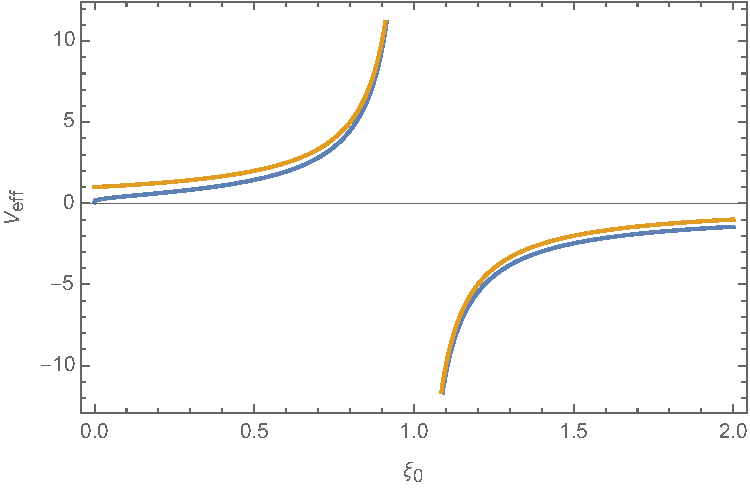
\includegraphics[width=0.55\linewidth]{./fig/fig_eq_10_11.pdf}
    \caption{The behaviour of $V_{eff}$ as the function of $\xi_0$. The yellow line is the approximation one.}%
    \label{fig:eq_10_1}
\end{figure}
The electrons near the Fermi energy will interact with their pair on the opposite side of the Fermi sea.
The mutual scattering produces a pole in the scattering amplitude, which will make the pair of electrons try to bind together.
The entire electron paires are doing this simultaneously, so that the entire metal undergoes a phase transition.
The existence of this pole depended on the sharpness of the electron distribution.
If all the electrons near the Fermi energy become paired, one must reconsider wheter this sharp distribution still exits.
A theory of superconducitivity must self-consistently determin the properties of bound electron pairs.

Another way to describe the instability is as a function of temperature.
It enters into the electron distribution $\eta_F$ by changing the step function into a smooth function with an energy width of severla $k_B T$.
By expressing the \eqref{10.5} as
\begin{equation}
    \int_{-\omega_D}^{\omega_D} d\xi_1 \frac{\eta_F(\xi_1)}{\xi-\xi_1} \approx  - \frac{1}{2} \ln \left[ \frac{\xi^2 + (k_B T)^2}{\omega_D^2}  \right] \label{10.12}
\end{equation}
Summation of all the ladder diagrams and the effectivce potential have the form
\begin{equation}
    V_{eff} = - \frac{V_0}{1+ N_F V_0 \ln \left[ \sqrt{\xi^2 + (k_BT)^2}/\omega_D  \right]}     \label{10.13}
\end{equation}
At zero energy, $\xi=0$, $V_{eff}$ becomes sigular when the temperature is lower to the critical temperature $T_c$
\begin{equation}
    k_B T_c = \omega_D \exp \left[ - \frac{1}{N_F V_0} \right]  \label{10.14}
\end{equation}

The theory of Cooper instability should be compared, for example, with the ordinary binding of two isolated particles.
If two particles are isolated, they do not have to obey the statistics of a collection of identical particles.
Then the stattering theory does not contain any of the occupation factors. all states may be used as intermediate state since there are no other particles.
In theory of Wannier excitons \ref{se:9.2}, the multiple scattering theory may be described by a vertex function
\begin{equation}
    \Gamma(\bk,\bk') = V(\bk-\bk') + \int \frac{d^3 k_1}{(2\pi)^3} \frac{V(\bk-\bk_1) \Gamma(\bk_1,\bk')}{2\xi_\bk - 2\xi_{\bk_1}}  \label{10.16}
\end{equation}
The solution to this vertex function is equivalent to solving the two-particle Schr{\"o}dinger equation in relative coordinates
\begin{equation}
    \left[- \frac{1}{2m} \left(\nabla_1^2 + \nabla_2^2 \right) + V(\br_1 -\br_2) -E \right] \psi(\br_1,\br_2) = 0   \label{10.17}
\end{equation}
The problem is factored into the relative and center of mass motions
\begin{eqnarray}
    \br &=& \br_1 - \br_2, ~ ~ ~ \psi(\br_1,\br_2) = e^{i \bp \cdot \mathbf{R}} \phi(\br) \label{10.18}\\
    \mathbf{R} &=& \frac{1}{2} (\br_1 + \br_2), ~ ~ ~ E= \frac{p^2}{2m} + \varepsilon   \label{10.19} \\
    &&\left[ - \frac{\nabla^2}{m} + V(\br) - \varepsilon \right] \phi(\br) = 0 \label{10.20}
\end{eqnarray}
The center of mass motion is plane wave, and the relative motion becomes a one-body problem.
Without the occupation factors, the relative scattering of two particles by an instantaneous potential is a trival problem.
When bound states occur, they are at negative binding energy in the relative coordinates, $\varepsilon<0$.
This behaviour is great contrast to the Cooper instability, where the pole occurs at small negative energy relative the to $E_F$, so the pole is at a positive energy $E_F-\xi_0$.
The two electrons cannot really bind at that neregy, since their net energy is positive.
\textit{The instability occurs because it appears to them as if they should bind, although if they tried, they would find they could not.}
The role of the occupation factors in the argument of the scattering integral is what moved the apparent pole out to the Fermi energy.\footnote{The reason electrons must be paired with opposite momentum, P633}

\subsection{BCS Theory}
The basic feature of the BCS theory is that pairing occurs between electrons in states with opposite momentum ans opposite spins.
The two spins are combined into a spin singlet, with $S=0$.
